\documentclass[10pt,journal,compsoc]{IEEEtran}

% Revised for IEEE Computer, September 2026.
% Compile with pdfLaTeX twice. Self-contained: all figures are drawn in LaTeX
% and all results are written in the text (from final_analysis.py).
%TC:group thebibliography 1 1
%TC:group IEEEbiographynophoto 1 1
%TC:group tabular 0 1
%TC:macro \mgsection [header]
%TC:macro \mgsub [header]
%TC:macro \IEEEPARstart [text,text]
\usepackage{graphicx}
\usepackage{tikz}
\usepackage{pgfplots}
\usepackage{booktabs}
\usetikzlibrary{patterns}
\pgfplotsset{compat=1.17}
\usetikzlibrary{arrows.meta}

\definecolor{pcInk}{HTML}{18212E}
\definecolor{pcBlue}{HTML}{306A9E}
\definecolor{pcPurple}{HTML}{795DA1}
\definecolor{pcAmber}{HTML}{A86108}
\definecolor{pcRed}{HTML}{A63238}
\definecolor{pcGreen}{HTML}{21643C}
\usepackage[T1]{fontenc}
\usepackage[utf8]{inputenc}
\usepackage[american]{babel}
\usepackage[super,nocompress]{cite}
\graphicspath{{figures/}{Images/}{images/}{./}}
\usepackage{microtype}
\usepackage{listings}
\usepackage{tcolorbox}
\tcbuselibrary{skins,breakable}
\usepackage{xurl}
\usepackage[hidelinks]{hyperref}

\setcounter{dbltopnumber}{2}
\renewcommand{\dbltopfraction}{0.9}
\renewcommand{\dblfloatpagefraction}{0.7}
\setcounter{secnumdepth}{0}
\newcommand{\mgsection}[1]{\section*{\MakeUppercase{#1}}}
\newcommand{\mgsub}[1]{\subsection*{#1}}
\newtcolorbox{mgbox}[1]{%
  breakable=false, colback=white, colframe=black,
  fonttitle=\bfseries\sffamily,
  title={\MakeUppercase{#1}}, boxrule=0.4pt, arc=0pt,
  left=7pt, right=7pt, top=6pt, bottom=6pt}
\lstset{
  basicstyle=\ttfamily\footnotesize,
  breaklines=true, numbers=none,
  frame=none, columns=fullflexible, keepspaces=true,
  showstringspaces=false}


% ---- Paste your public repository URL between the braces (leave empty to hide the link):
\def\RepoURL{}

\begin{document}

\title{What Did This Patch Remove?}
% Alternative title (6 words): What Did Your AI Patch Remove?

\author{%
  Bilal~Sardar,\;\textit{LUT University}\quad
  Prabhat~Kumar,\;\textit{LUT University}\\[2pt]
  Ankit~Agrawal,\;\textit{LUT University}\quad
  Najmul~Islam,\;\textit{LUT University}%
  \IEEEcompsocitemizethanks{%
    \IEEEcompsocthanksitem Corresponding author: B. Sardar,
      bilal.sardar@lut.fi}}

\markboth{Computer}{Sardar \MakeLowercase{\textit{et al.}}: What Did This Patch Remove?}

\IEEEtitleabstractindextext{%
\begin{abstract}
A leaderboard counts a patch as resolved when its target tests pass; merging it
depends on everything else it changed. We examined 3,284 test-passing patches
from 11 public AI agent configurations (2024--2026) alongside developers' fixes
for the same issues. The 2024 agent designs left stray files in 35 percent of
resolved patches, and one rewrote existing tests. About one patch in 40 removed
a guard, a validation call, an error path, or a test. Blind labeling found most
removals were the intended fix, but two were harmful: a developer's dropped
validation and an agent's deleted path-traversal test. Nothing in the usual
pipeline reported either. Matched by issue, agents removed protections no more
often than developers, so the gap lies in review, not in AI. We propose a
removal report for every patch, and PATCH, a review loop built around it.
\end{abstract}

\begin{IEEEkeywords}
Automated program repair, AI-generated code, software security, coding agents,
code review, patch validation.
\end{IEEEkeywords}}

\maketitle
\IEEEdisplaynontitleabstractindextext
\IEEEpeerreviewmaketitle

\IEEEPARstart{A}{n} AI agent reads an issue, edits the code, and runs the tests.
The build turns green, the agent explains its change, and a leaderboard counts
the issue as resolved. What nobody has checked is what the patch took away.

Language models now resolve real GitHub issues,\cite{jimenez2024swebench} and an
earlier \emph{Computer} article asked how well they repair buggy
code.\cite{zhang2025canai} The usual worry is that AI writes less secure fixes
than people do, and earlier studies report worrying rates of new weaknesses in
model-written fixes.\cite{sajadi2025howsafe,hoodlet2026flawed} We asked a
different question: when a test-passing patch is merged, what does it remove,
and does anything in the review pipeline notice?

Program-repair research has known for a decade that a patch can pass its tests
by deleting functionality,\cite{qi2015plausibility} and recent work shows that
``resolved'' on SWE-bench overstates correctness.\cite{wang2026solved,aleithan2024swebenchplus}
We call the security side of this the \emph{absence problem}. It applies to
every patch, whoever wrote it. What AI changes is the rate at which patches
arrive: agents can produce candidate fixes faster than teams can review them,
each with a fluent explanation of what it added.

This article makes three contributions. We measure what 3,284 public
test-passing patches carried besides their fix, compared issue by issue with
developers' fixes and checked by blind labeling. We show that no stage of the
usual pipeline reports a removal. And we propose a removal report for every
patch, with PATCH, a lightweight review loop built around it, and measure how
often it would ask a reviewer for attention.

\mgsection{The absence problem}

Tests run code on chosen inputs; static analyzers match patterns in code. Both
examine what the patch leaves in place. When a patch adds an \texttt{eval} call
or builds SQL from strings, there is something to find, and scanners usually
find it. When a patch deletes a guard clause, drops a validation call, swallows
an exception, or trims a test, nothing remains to run or to match
(Figure~\ref{fig:concept}). That is how the tools are designed, not a defect in
them. The question is whether anything else in the pipeline accounts for what
was removed. Diff views draw the eye to new code, and an agent's explanation
describes what it added, which is a claim about the change rather than evidence
that every protection survived.

Removal is not always wrong. Often it is the fix: an issue may ask for an error
to stop being raised. So the goal is not to forbid removals but to account for
each one, showing that what was removed is no longer needed or is enforced
somewhere else.

\begin{figure*}[t]
\centering
\resizebox{\textwidth}{!}{%
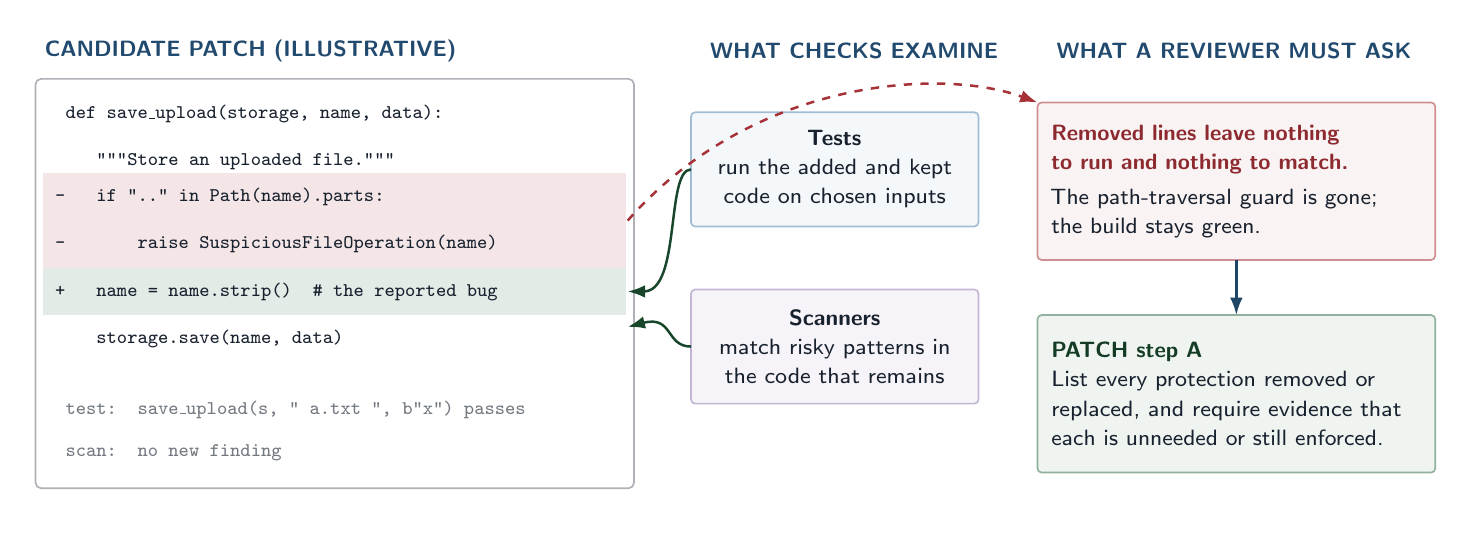
\begin{tikzpicture}[
  x=1cm,y=1cm,
  font=\sffamily\fontsize{8.5}{10.5}\selectfont,
  every node/.style={text=pcInk,align=center,outer sep=0pt},
  box/.style={rounded corners=1.5pt,line width=0.6pt,draw=pcBlue!45,fill=pcBlue!5,inner sep=5pt},
  code/.style={anchor=west,font=\ttfamily\fontsize{7.2}{9}\selectfont,inner sep=0pt},
  head/.style={anchor=west,font=\sffamily\bfseries\fontsize{8.5}{10}\selectfont,text=pcBlue!70!black},
  flow/.style={-{Latex[length=2.2mm,width=1.6mm]},line width=0.9pt}
]
\path[use as bounding box] (0,0) rectangle (18,6.4);
\node[head] at (0.1,6.1) {CANDIDATE PATCH (ILLUSTRATIVE)};
\node[head] at (8.55,6.1) {WHAT CHECKS EXAMINE};
\node[head] at (12.95,6.1) {WHAT A REVIEWER MUST ASK};
% diff card
\draw[rounded corners=2pt,line width=0.6pt,draw=pcInk!35,fill=white] (0.1,0.55) rectangle (7.7,5.75);
\fill[pcRed!12] (0.2,3.95) rectangle (7.6,4.55);
\fill[pcRed!12] (0.2,3.35) rectangle (7.6,3.95);
\fill[pcGreen!13] (0.2,2.75) rectangle (7.6,3.35);
\node[code] at (0.35,5.3) {\ def save\_upload(storage, name, data):};
\node[code] at (0.35,4.7) {\ \ \ \ """Store an uploaded file."""};
\node[code] at (0.35,4.25) {-\ \ \ if ".." in Path(name).parts:};
\node[code] at (0.35,3.65) {-\ \ \ \ \ \ \ raise SuspiciousFileOperation(name)};
\node[code] at (0.35,3.05) {+\ \ \ name = name.strip() \ \# the reported bug};
\node[code] at (0.35,2.45) {\ \ \ \ storage.save(name, data)};
\node[code,text=pcInk!60] at (0.35,1.55) {\ test: save\_upload(s, " a.txt ", b"x") passes};
\node[code,text=pcInk!60] at (0.35,1.0) {\ scan: no new finding};
% checks
\node[box,text width=3.3cm,minimum height=1.45cm] (tests) at (10.25,4.6)
  {\textbf{Tests}\\run the added and kept\\code on chosen inputs};
\node[box,draw=pcPurple!45,fill=pcPurple!7,text width=3.3cm,minimum height=1.45cm] (scan) at (10.25,2.35)
  {\textbf{Scanners}\\match risky patterns in\\the code that remains};
\draw[flow,draw=pcGreen!70!black] (tests.west) .. controls (8.1,4.6) and (8.3,3.05) .. (7.62,3.05);
\draw[flow,draw=pcGreen!70!black] (scan.west) .. controls (8.1,2.35) and (8.2,2.75) .. (7.62,2.6);
% right boxes
\node[box,draw=pcRed!55,fill=pcRed!6,text width=4.7cm,minimum height=2.0cm,align=left] (gap) at (15.35,4.45)
  {{\color{pcRed!85!black}\bfseries Removed lines leave nothing}\\{\color{pcRed!85!black}\bfseries to run and nothing to match.}\\[2pt]
   The path-traversal guard is gone;\\ the build stays green.};
\node[box,draw=pcGreen!50,fill=pcGreen!7,text width=4.7cm,minimum height=2.0cm,align=left] (ask) at (15.35,1.75)
  {{\color{pcGreen!60!black}\bfseries PATCH step A}\\
   List every protection removed or replaced, and require evidence that each is unneeded or still enforced.};
\draw[flow,draw=pcRed,dashed] (7.62,3.95) .. controls (9.2,5.75) and (11.6,5.9) .. (gap.north west);
\draw[flow,draw=pcBlue!65!black] (gap.south) -- (ask.north);
\end{tikzpicture}%
}
\caption{The absence problem. Tests and scanners examine the code a patch adds
or keeps. A patch that deletes a protection while fixing the reported bug passes
both, because nothing is left for either check to see. The example is
illustrative; the sidebar describes a real case.}
\label{fig:concept}
\end{figure*}

\mgsection{What earlier work found}

Table~\ref{tab:evidence} summarizes recent studies of AI repair and security,
together with two strands this article builds on: patches that pass tests by
deleting functionality,\cite{qi2015plausibility} and resolved benchmark issues
that are not really solved.\cite{wang2026solved,aleithan2024swebenchplus} The
studies differ in task, population, and evaluation, so their numbers cannot be
pooled. Together they show that tests accept patches that do less than intended,
that new weaknesses can differ in kind from the bug being fixed, and that
crafted issue reports can steer agents. None measures, at agent scale and
against developers' fixes, what test-passing patches remove and whether
anything reports it.

\begin{table*}[t]
\centering
\caption{Related evidence, as reported by each study. Populations and measures
differ, so rows are not comparable as risk rates.}
\label{tab:evidence}
\footnotesize
\renewcommand{\arraystretch}{1.16}
\begin{tabular}{@{}p{2.5cm}p{4.3cm}p{5.4cm}p{4.4cm}@{}}
\toprule
\textbf{Study} & \textbf{Setting} & \textbf{Key finding} & \textbf{Limits}\\
\midrule
Qi et al.\cite{qi2015plausibility} & Three generate-and-validate repair systems
 & Most test-passing patches incorrect; a repair tool that only deletes functionality performed comparably
 & Pre-LLM tools; correctness, not security \\
Wang et al.;\cite{wang2026solved} Aleithan et al.\cite{aleithan2024swebenchplus} & Agent patches on SWE-bench
 & Resolved rates inflated: validation skips unchanged test files; weak tests accept wrong patches
 & Correctness, not security \\
Sajadi et al.\cite{sajadi2025howsafe} & Llama 3.3 vs.\ developers on 20,000+ SWE-bench issues; three agents
 & 135 vs.\ 12 new vulnerabilities after tool voting and manual review; weaknesses cluster in runaway attempts
 & Counts added weaknesses; model rewrote whole files \\
Shukla et al.\cite{shukla2025degradation} & 400 samples ``improved'' over repeated rounds
 & Mean vulnerabilities rose from 2.1 early to 6.2 by rounds 8--10
 & Unattended refinement, not issue repair \\
Przymus et al.;\cite{przymus2026adversarial} Chen et al.\cite{chen2026redteaming} & 51 crafted bug reports; red-teamed repair agents
 & 90\% attacker-aligned patches; steered patches passed tests yet were vulnerable
 & Crafted attacks \\
Mierczuk et al.\cite{hoodlet2026flawed} & ChatGPT 5.5 and Claude Opus 4.8 on six recent vulnerabilities
 & 26.0\% of 6,080 attempts were complete, behavior-preserving fixes
 & Industry report; model-graded \\
This article & 11 agent configurations, SWE-bench Verified, 2024--2026
 & About 1 in 40 resolved patches removed a protection or test; 2 of 97 removals harmful; none reported by tests or scanners
 & Python; ordinary bug fixes \\
\bottomrule
\end{tabular}
\end{table*}

\mgsection{What we measured}

We analyzed public patches, so anyone can repeat the study. SWE-bench Verified
holds 500 human-validated issues from 12 Python projects,\cite{chowdhury2024verified}
and its leaderboard archives each entry's patches and test results.\cite{swebench2026experiments}
We took every patch the benchmark counts as resolved from two cohorts chosen so
that one varies the agent and the other varies the model: five widely used
agent designs built on Claude~3.5 Sonnet in 2024, and one minimal scaffold,
mini-SWE-agent,\cite{yang2024sweagent} run with six frontier and open-weight
models released between August 2025 and May 2026. The scaffold version differs
between entries (Table~\ref{tab:results}), so model comparisons are descriptive.
We excluded two further entries for which too few resolved patches could be
retrieved and applied: Claude Sonnet 4 (35 percent) and Kimi K2.5 (28 percent).
Developers' fixes are the baseline, always compared on the issues each
configuration resolved.

For each patch we compared every changed function before and after. We recorded
\emph{removals}---a guard clause that raises, a validation, escaping, or
permission call, an error now swallowed by a broad exception handler, or an
assertion deleted from an existing test---and \emph{additions} of risky
operations such as \texttt{eval}, unsafe deserialization, shell commands, or SQL
built from strings. Bandit and Semgrep ran on every changed production file
before and after, keeping new findings of medium or higher severity. Any
removal, addition, or new finding held a patch for a security-focused look. To
check the detector, we deleted one protection from each developer's fix that
allowed it; it flagged 99 percent of these 832 seeded deletions.

Two authors then labeled every removal from a written four-category guide:
harmful to security and not called for by the issue, questionable, intended by
the issue, or unsure. Each worked separately, without knowing whether an agent
or a developer wrote the patch and before any discussion, although stray files
or coding style could sometimes reveal an agent.
% CHECK before submission: confirm A1 and A2 were labeled independently (their notes differ).

\begin{table*}[t]
\centering
\caption{Test-passing (resolved) patches on SWE-bench Verified. Held: any
removal, risky addition, or new scanner finding (95\% Wilson interval).
Developers, same issues: held rate of developers' fixes for exactly the issues
that configuration resolved. Removal: share of patches with at least one. Stray:
patches that add new Python files outside the project's source directories.
Date: entry date (upper group) or model release (lower group); the lower group
uses mini-SWE-agent, with its version in parentheses.}
\label{tab:results}
\footnotesize
\renewcommand{\arraystretch}{1.12}
\begin{tabular}{@{}lcrcccc@{}}
\toprule
\textbf{Configuration} & \textbf{Date} & \textbf{Patches} & \textbf{Held, \% (95\% CI)} &
\textbf{Developers, same issues, \%} & \textbf{Removal, \%} & \textbf{Stray, \%}\\
\midrule
\textit{Developer fixes (all)} & -- & 500 & 5.4 (3.7--7.7) & -- & 3.6 & 0 \\
\midrule
SWE-agent & 2024-06 & 168 & 12.5 (8.3--18.4) & 6.0 & 10.1 & 44 \\
Minimal tools & 2024-10 & 244 & 4.1 (2.2--7.4) & 4.9 & 2.5 & 80 \\
OpenHands & 2024-10 & 240 & 4.6 (2.6--8.0) & 4.2 & 2.5 & 55 \\
AutoCodeRover & 2024-11 & 231 & 3.0 (1.5--6.1) & 5.2 & 2.2 & 0 \\
Agentless & 2024-12 & 254 & 3.5 (1.9--6.6) & 6.3 & 2.4 & 0 \\
\midrule
GPT-5 (v1.7) & 2025-08 & 314 & 5.1 (3.2--8.1) & 4.8 & 4.1 & 2 \\
Claude Opus 4.5 (v1.16) & 2025-11 & 372 & 3.2 (1.9--5.6) & 4.8 & 1.3 & 1 \\
GPT-5.2 (v2.0) & 2025-12 & 364 & 4.1 (2.5--6.7) & 4.1 & 1.9 & 0 \\
Claude Opus 4.6 (v2.0) & 2026-02 & 378 & 2.9 (1.6--5.1) & 4.8 & 1.3 & 0 \\
GLM-5 (v2.0) & 2026-02 & 360 & 2.2 (1.1--4.3) & 5.3 & 0.8 & 0 \\
Gemini 3.5 Flash (v2.4) & 2026-05 & 359 & 4.2 (2.5--6.8) & 4.7 & 1.7 & 0 \\
\bottomrule
\end{tabular}
\end{table*}

\begin{figure*}[t]
\centering
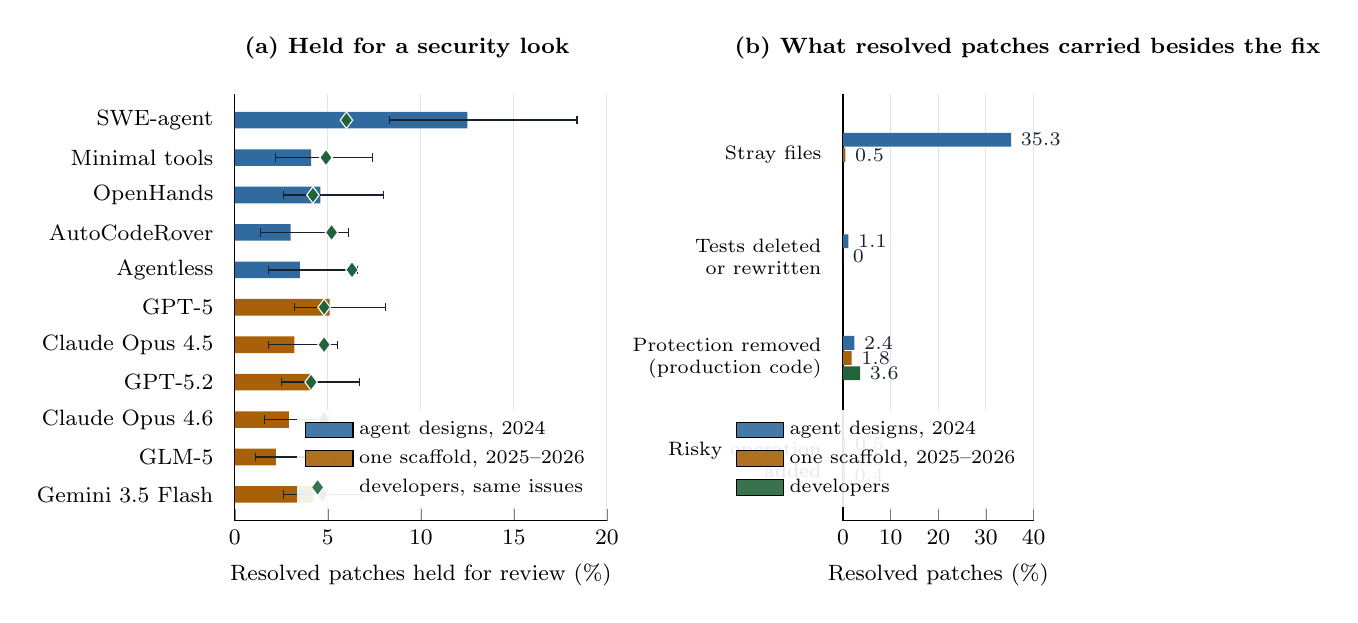
\begin{tikzpicture}
\begin{axis}[
  name=pa, width=0.52\textwidth, height=7.0cm, xbar, bar width=6pt, bar shift=0pt,
  xmin=0, xmax=20, ymin=0.3, ymax=11.7, y dir=reverse,
  ytick={1,...,11}, yticklabels={SWE-agent,Minimal tools,OpenHands,AutoCodeRover,Agentless,GPT-5,Claude Opus 4.5,GPT-5.2,Claude Opus 4.6,GLM-5,Gemini 3.5 Flash}, ytick style={draw=none},
  xlabel={Resolved patches held for review (\%)}, xmajorgrids, grid style={pcInk!12},
  axis x line*=bottom, axis y line*=left, tick label style={font=\footnotesize},
  label style={font=\footnotesize},
  title={\textbf{(a) Held for a security look}}, title style={font=\footnotesize, align=left, at={(0,1.02)}, anchor=south west},
  legend style={font=\scriptsize, draw=none, fill=white, fill opacity=0.9, text opacity=1, at={(0.98,0.03)}, anchor=south east, cells={anchor=west}},
  error bars/error bar style={pcInk, line width=0.5pt}, error bars/error mark options={rotate=90, mark size=1.5pt, pcInk}]
\addplot[draw=none, fill=pcBlue, area legend, error bars/.cd, x dir=both, x explicit] coordinates {(12.5,1) += (5.9,0) -= (4.2,0) (4.1,2) += (3.3,0) -= (1.9,0) (4.6,3) += (3.4,0) -= (2.0,0) (3.0,4) += (3.1,0) -= (1.6,0) (3.5,5) += (3.1,0) -= (1.7,0)};
\addlegendentry{agent designs, 2024}
\addplot[draw=none, fill=pcAmber, area legend, error bars/.cd, x dir=both, x explicit] coordinates {(5.1,6) += (3.0,0) -= (1.9,0) (3.2,7) += (2.3,0) -= (1.4,0) (4.1,8) += (2.6,0) -= (1.6,0) (2.9,9) += (2.2,0) -= (1.3,0) (2.2,10) += (2.1,0) -= (1.1,0) (4.2,11) += (2.6,0) -= (1.6,0)};
\addlegendentry{one scaffold, 2025--2026}
\addplot[only marks, mark=diamond*, mark size=3pt, color=pcGreen, mark options={draw=white, line width=0.4pt}, legend image code/.code={\draw[mark repeat=2, mark phase=2] plot coordinates {(0cm,0cm) (0.15cm,0cm) (0.3cm,0cm)};}] coordinates {(6.0,1) (4.9,2) (4.2,3) (5.2,4) (6.3,5) (4.8,6) (4.8,7) (4.1,8) (4.8,9) (5.3,10) (4.7,11)};
\addlegendentry{developers, same issues}
\end{axis}
\begin{axis}[
  at={(pa.east)}, anchor=west, xshift=3.0cm, width=0.33\textwidth, height=7.0cm,
  xbar, bar width=5pt, xmin=0, xmax=40, ymin=0.4, ymax=4.6, y dir=reverse,
  ytick={1,2,3,4}, yticklabels={{Stray files},{Tests deleted\\or rewritten},{Protection removed\\(production code)},{Risky operation\\added}},
  yticklabel style={align=right, font=\scriptsize}, ytick style={draw=none},
  xlabel={Resolved patches (\%)}, xmajorgrids, grid style={pcInk!12},
  axis x line*=bottom, axis y line*=left, tick label style={font=\footnotesize}, label style={font=\footnotesize},
  nodes near coords={\pgfmathprintnumber[fixed,precision=1]{\pgfplotspointmeta}},
  nodes near coords style={font=\scriptsize, text=pcInk, anchor=west},
  legend style={font=\scriptsize, draw=none, fill=white, fill opacity=0.9, text opacity=1, at={(0.98,0.03)}, anchor=south east, cells={anchor=west}},
  title={\textbf{(b) What resolved patches carried besides the fix}}, title style={font=\footnotesize, align=left, at={(-0.62,1.02)}, anchor=south west}]
\addplot[draw=none, fill=pcBlue, bar shift=5.5pt, area legend] coordinates {(35.3,1) (1.1,2) (2.4,3) (0.5,4)};
\addlegendentry{agent designs, 2024}
\addplot[draw=none, fill=pcAmber, bar shift=0pt, area legend] coordinates {(0.5,1) (0.0,2) (1.8,3) (0.5,4)};
\addlegendentry{one scaffold, 2025--2026}
\addplot[draw=none, fill=pcGreen, bar shift=-5.5pt, area legend] coordinates {(3.6,3) (0.4,4)};
\addlegendentry{developers}
\end{axis}
\end{tikzpicture}
\caption{(a) Share of test-passing patches the automated triage held for a
security-focused look (bars, 95\% Wilson intervals) and the same share for
developers' fixes to exactly those issues (diamonds). Only SWE-agent, which
rewrote tests, was held clearly more often. (b) What resolved patches contained
besides the fix, for the 2024 agent designs (blue, 1,137 patches), the
2025--2026 scaffold (amber, 2,147), and developers' fixes (green, 500).
Developers' fixes contain no test changes and no stray files, so they have no
bars in the first two rows.}
\label{fig:results}
\end{figure*}

\mgsub{What resolved patches carried}
Resolved patches often carried more than their fix (Figure~\ref{fig:results}b).
The 2024 agent designs left stray Python files, such as reproduction scripts, in
35 percent of resolved patches (up to 80 percent for one design), against 0.5
percent for the newer scaffold; one patch also committed a SQLite database file.
SWE-agent edited or deleted existing test assertions in 13 of its 168 resolved
patches. In 14 patches, agents added a broad exception handler that silently
discards errors, which developers' fixes never did, and one fixed an ordering bug
by assembling raw SQL from string fragments. Across all 3,784 patches, 97
removed a protection or a test: 84 in production code (51 guard clauses, 21
validation, escaping, or permission calls, and 14 newly silenced errors; two
patches did two of these) and 13 only in tests.

\mgsub{Matched by issue, agents removed no more than developers}
Of 3,284 resolved agent patches for 442 issues, 4.1 percent were held, and ten
of eleven configurations were held no more often than developers' fixes for the
same issues (Table~\ref{tab:results}, Figure~\ref{fig:results}a). The exception
was SWE-agent, held in 12.5 percent of patches against 6.0 percent for
developers on its issues (difference 6.5 points, 95 percent interval 1.8 to
11.9), mostly because it rewrote tests. Pooled over all eleven, agents were held
0.8 points less often than developers (interval $-2.3$ to 0.5, resampling whole
issues). Holds for 2025--2026 models ranged from 2.2 to 5.1 percent, with no
trend across generations. Sajadi and colleagues counted new weaknesses a model
added;\cite{sajadi2025howsafe} we count what patches removed, so the two studies
measure different things.

\mgsub{Which removals mattered}
The two labelers agreed on all 97 removals before any discussion (Cohen's
$\kappa$ = 1.00). The agreement reflects how clear-cut most cases were: 93
removals were plainly the fix the issue asked for. Two were unexplained test
rewrites a maintainer should question. Two removed a security-relevant
protection the issue did not call for. In one, a developer's own merged fix
dropped a validation call and a guard from production code. In the other, an
agent deleted a path-traversal test in a patch the leaderboard counted as
resolved (see the sidebar). As a check on the labels, Claude Sonnet 5.5 labeled
the same patches from the same guide. It found one of the two harmful removals
and questioned 27 of the 93 intended ones, so its judgments would still need a
person to confirm them.
\IfFileExists{paper_a3.tex}{\input{paper_a3.tex}}{}

\mgsub{Nothing in the pipeline reported them}
Every one of the 97 removals, including both harmful ones, passed the
benchmark's tests. The scanners flagged 14 of 18 patches that added a risky
operation and none of the 84 that removed a protection from production code;
they do not read tests, so the 13 test deletions were outside their reach, and
a green run cannot report a test that no longer exists. The leaderboard reports
whether the target tests pass, not what else changed, as earlier work also
found.\cite{wang2026solved} Each tool behaved as designed. No stage asked what
the patch removed.

\mgsub{What a removal report costs}
Our automated triage held 4.1 percent of agent patches for a security-focused
look, and another 17 percent raised only scope triggers, mostly stray files; in
all, about one patch in five would ask a reviewer for some attention. Of the 97
removals it listed, 93 needed only a one-line justification.
\IfFileExists{paper_misscheck.tex}{\input{paper_misscheck.tex}}{}

These results have limits. They cover Python projects in one curated benchmark
with known contamination and test-adequacy concerns,\cite{aleithan2024swebenchplus}
chosen because its patches, tests, and developers' fixes are public. Both
labelers are authors.\IfFileExists{paper_a3.tex}{}{ A non-author labeler would
strengthen the labels.} The labels show which removals mattered, not whether an
attacker could exploit them. Our lists of protections and risky operations are
deliberately simple, so the counts are lower bounds; they miss, for example, a
check that is kept but loosened.\IfFileExists{paper_misscheck.tex}{}{ We have
not measured how many removals the detector misses in patches it let through.}
The study covers ordinary bug fixes; vulnerability repairs, where every removal
matters, deserve the same measurement.

\begin{mgbox}{A resolved patch that deleted a security test}
\small
A Django issue reported that a \texttt{FileField} with callable storage was
serialized incorrectly into migrations. SWE-agent with Claude~3.5 Sonnet fixed
it by changing one condition. The same patch rewrote the field's test module,
replacing 13 existing tests with one new test. Among those deleted:
\begin{lstlisting}[language=Python]
-    def test_save_without_name(self):
-        ...
-            msg = f"Detected path traversal attempt in '{tmp.name}'"
-            with self.assertRaisesMessage(SuspiciousFileOperation, msg):
-                document.save()
\end{lstlisting}
The benchmark counted the patch as resolved. A green run cannot report a test
that no longer exists, and scanners do not read tests; a coverage or mutation
comparison could have noticed. Merged, the fix would have worked, and the project
would have silently lost its test that saving a file cannot escape the storage
directory.

\textbf{Review question:} Which tests did this patch remove, and why?
\end{mgbox}

\mgsection{A removal report, and a loop around it}

Our central proposal is simple: every patch, human or AI, should come with a
\emph{removal report} that lists each guard, validation or permission call,
error path, test, and library abstraction it removed or routed around, and
states either why the issue requires the removal or where the protection is
now enforced. PATCH places that report in a five-step review loop
(Figure~\ref{fig:patch}). Only step A is new; the other steps restate
established practice so a team can adopt the report without redesigning its
review. PATCH complements secure development guidance such as NIST's profile for
generative AI\cite{booth2024ssdf} by narrowing to one decision: whether to merge
a specific candidate. We offer it as a proposal; the human steps still need
evaluation with working reviewers.

\begin{figure*}[!t]
\centering
\resizebox{\textwidth}{!}{%
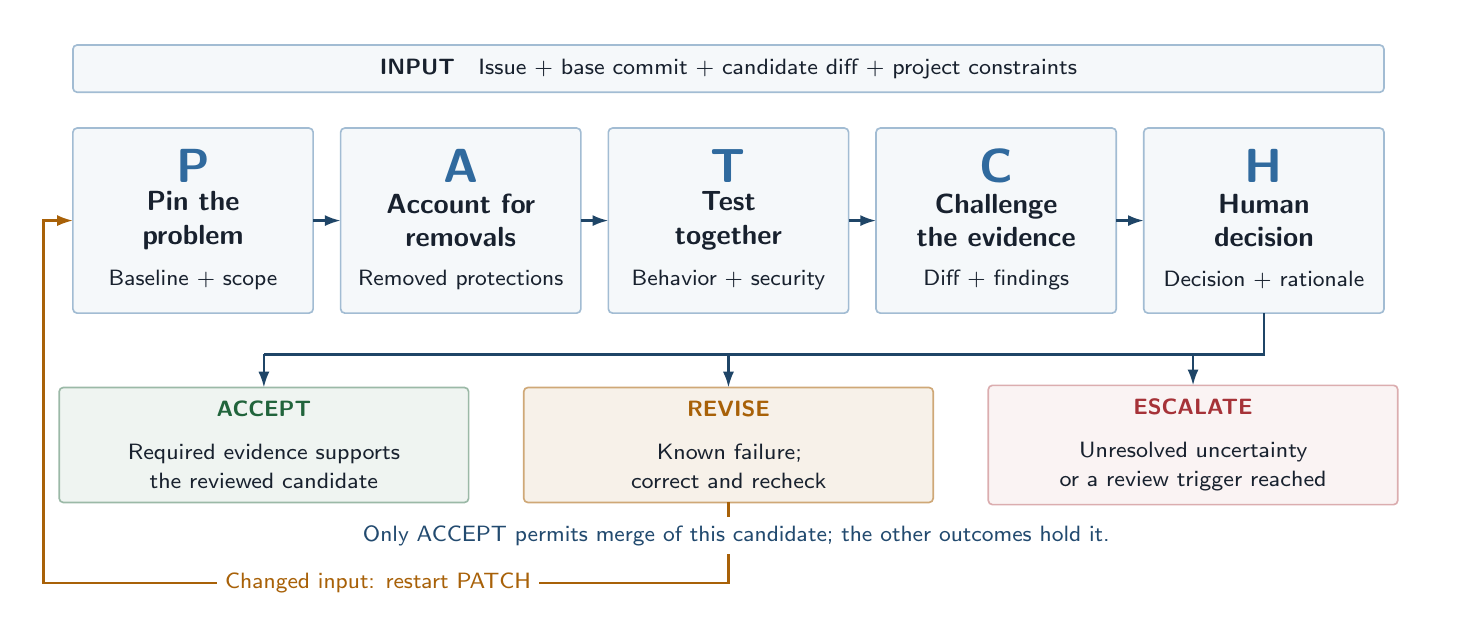
\begin{tikzpicture}[
  x=1cm,y=1cm,
  font=\sffamily\fontsize{8.5}{10.5}\selectfont,
  every node/.style={
    text=pcInk,align=center,outer sep=0pt
  },
  box/.style={
    rounded corners=1.5pt,
    line width=0.6pt,
    draw=pcBlue!45,
    fill=pcBlue!5
  },
  stage/.style={
    box,
    text width=2.77cm,
    minimum width=3.05cm,
    minimum height=2.35cm,
    inner sep=4pt
  },
  decision/.style={
    box,
    text width=4.8cm,
    minimum width=5.2cm,
    minimum height=1.45cm,
    inner sep=5pt
  },
  flow/.style={
    -{Latex[length=2mm,width=1.4mm]},
    draw=pcBlue!65!black,
    line width=0.8pt
  },
  letter/.style={
    text=pcBlue,
    font=\sffamily\bfseries\fontsize{17}{19}\selectfont
  },
  detail/.style={
    font=\sffamily\fontsize{8}{10}\selectfont
  }
]
\path[use as bounding box] (0,0) rectangle (18,7.4);

% Input to the review
\node[
  box,
  text width=16.25cm,
  minimum width=16.65cm,
  minimum height=0.6cm,
  inner sep=4pt
] at (8.90,6.88)
  {\textbf{INPUT}\quad
   Issue + base commit + candidate diff + project constraints};

% Five stage cards
\foreach \name/\x in {
  P/2.10,
  A/5.50,
  T/8.90,
  C/12.30,
  H/15.70
}{
  \node[stage] (\name) at (\x,4.95) {};
  \node[letter] at (\x,5.65) {\name};
}

% Stage titles
\node[font=\sffamily\bfseries]
  at (2.10,4.95) {Pin the\\problem};

\node[font=\sffamily\bfseries]
  at (5.50,4.95) {Account for\\removals};

\node[font=\sffamily\bfseries]
  at (8.90,4.95) {Test\\together};

\node[font=\sffamily\bfseries]
  at (12.30,4.95) {Challenge\\the evidence};

\node[font=\sffamily\bfseries]
  at (15.70,4.95) {Human\\decision};

% Stage outputs
\node[detail] at (2.10,4.20)
  {Baseline + scope};

\node[detail] at (5.50,4.20)
  {Removed protections};

\node[detail] at (8.90,4.20)
  {Behavior + security};

\node[detail] at (12.30,4.20)
  {Diff + findings};

\node[detail] at (15.70,4.20)
  {Decision + rationale};

% Sequential review flow
\draw[flow] (P.east) -- (A.west);
\draw[flow] (A.east) -- (T.west);
\draw[flow] (T.east) -- (C.west);
\draw[flow] (C.east) -- (H.west);

% Three possible decisions
\node[
  decision,
  draw=pcGreen!45,
  fill=pcGreen!7
] (accept) at (3.00,2.10)
  {{\color{pcGreen}\bfseries ACCEPT}\\[5pt]
   Required evidence supports\\
   the reviewed candidate};

\node[
  decision,
  draw=pcAmber!55,
  fill=pcAmber!9
] (revise) at (8.90,2.10)
  {{\color{pcAmber}\bfseries REVISE}\\[5pt]
   Known failure;\\
   correct and recheck};

\node[
  decision,
  draw=pcRed!40,
  fill=pcRed!6
] (escalate) at (14.80,2.10)
  {{\color{pcRed}\bfseries ESCALATE}\\[5pt]
   Unresolved uncertainty\\
   or a review trigger reached};

% Human decision branches
\draw[pcBlue!65!black,line width=0.8pt]
  (H.south) -- (15.70,3.25) -- (3.00,3.25);

\draw[flow]
  (3.00,3.25) -- (accept.north);

\draw[flow]
  (8.90,3.25) -- (revise.north);

\draw[flow]
  (14.80,3.25) -- (escalate.north);

% Revision loop
\draw[flow,draw=pcAmber]
  (revise.south)
  -- (8.90,0.35)
  -- (0.20,0.35)
  -- (0.20,4.95)
  -- (P.west);

\node[
  fill=white,
  inner sep=3pt,
  text=pcAmber
] at (4.45,0.35)
  {Changed input: restart PATCH};

\node[
  fill=white,
  inner sep=3pt,
  text=pcBlue!70!black
] at (9.00,0.95)
  {Only ACCEPT permits merge of this candidate;
   the other outcomes hold it.};

\end{tikzpicture}%
}
\caption{The PATCH review loop. Each step leaves a record that links what the
patch changed---above all, what it removed---to evidence about the same candidate.
Steps P, A, and T can be partly automated, as in our study; a named reviewer makes
the H decision. Only ACCEPT permits merge; a changed input restarts the loop.}
\label{fig:patch}
\end{figure*}

\mgsub{P---Pin the problem and scope}
Record the expected behavior, base commit, and candidate. Treat the issue report
as input, not authority, since crafted reports can steer
agents,\cite{przymus2026adversarial} and flag scope triggers set from the
project's own history, such as new dependencies or stray files.

\mgsub{A---Account for what was removed}
Write the removal report. For each item, record why the issue requires it or the
property that must still hold---for example, that a file name cannot escape the
storage directory---and where that property is now enforced. The first pass is
easy to automate: comparing each changed function's guards, validation calls,
exception handlers, and assertions before and after took well under a second per
patch in our study.

\mgsub{T---Test function and security together}
Run the regression suite, rerun any deleted test against the new code, and
compare test coverage before and after, so a deleted or weakened test shows up
as a drop. Compare scans before and after with complementary analyzers.

\mgsub{C---Challenge the evidence}
Treat scanner silence as saying nothing about removals, and an agent's
explanation as a claim to verify. Ask whether the change removes the cause or
only blocks the example it was shown.

\mgsub{H---Human decision and record}
A named reviewer chooses \textbf{ACCEPT} when every item in the removal report is
justified or its property demonstrated, \textbf{REVISE} when a specific
correction is known, or \textbf{ESCALATE} when evidence is missing. An AI
assistant can draft the report; our labeling results suggest a person should
still sign it.

For the sidebar case, A lists 13 deleted tests, including the path-traversal
check. T reruns them and sees coverage drop; C asks why they were removed. The
outcome is REVISE: keep the one-line fix and restore the tests.

\mgsection{What should change}

\mgsub{For teams}
Require a removal report on every pull request, human or AI, and add a coverage
comparison to the gate so deleted tests cannot pass silently. Most patches have
nothing to report, and most listed removals need one sentence each.

\begin{mgbox}{A removal report for the sidebar patch}
\small
\textbf{Removed:} 13 tests in \texttt{test\_filefield.py}, including the
path-traversal check.\\
\textbf{Needed by the issue?} No; the issue concerns migration serialization.\\
\textbf{Property:} saving a file must not escape the storage directory.\\
\textbf{Evidence:} none in the candidate.\\
\textbf{Replaced:} one storage condition, broadened to cover callable storage.\\
\textbf{Evidence:} the benchmark's target tests pass.\\
\textbf{Decision:} REVISE---keep the fix, restore the deleted tests.
\end{mgbox}

\mgsub{For benchmarks and leaderboards}
Report, next to the resolved rate, how many resolved patches removed
protections, deleted or rewrote tests, or left stray files, and run the full
test suite rather than only the target tests. Agents are often compared by
leaderboard rank, so ``resolved'' should come closer to ``mergeable.''

\mgsub{For research}
Removal-aware analysis deserves tool support: checks that describe what a patch
no longer enforces, not only what it newly contains. Security properties stated
once, such as ``file names never escape the storage directory,'' could be
checked against every later patch, so a removal would fail a check instead of
passing silently. PATCH's human steps need a study with reviewers under
realistic time pressure, and the same measurement should be repeated on
vulnerability repairs\cite{xu2026architectures} and in languages beyond Python.

\mgsection{Account for removals}

For today's agents on ordinary bugs, matched issue by issue, we found that they
remove protections no more often than developers do. The gap is in the pipeline
both rely on. It was built to find what a patch adds, and in our data it said
nothing about 97 removals, including the two that mattered. As agents take on
more of the fixing and patches arrive faster, removals need to be accounted for,
not merely noticed. Before merging any patch, a reviewer should be able to
answer three questions: What did this patch fix, what did it remove, and what
shows that the removed protection is no longer needed?

\mgsection{Data availability}

% The first sentence switches automatically once \RepoURL is set at the top of this file.
% With a Zenodo DOI as well, add: "An archived copy is at https://doi.org/10.5281/zenodo.XXXXXXX."
\ifx\RepoURL\empty
The analysis notebook, scripts, per-patch results, and labels are available from
the corresponding author and will be deposited in a public archive on
publication.
\else
The analysis notebook, scripts, per-patch results, labeling guide, and labels
are available at \expandafter\url\expandafter{\RepoURL}.
\fi
All patches analyzed are public artifacts of the SWE-bench
leaderboard.\cite{swebench2026experiments}

\mgsection{Acknowledgment}

% CHECK: make this statement match exactly what happened before submission.
Generative AI tools assisted with language editing, figure preparation, drafting
parts of the text and of the PATCH workflow, and writing the analysis code.
Claude Sonnet 5.5 (Anthropic; run on 29 September 2026) labeled the removal
patches as a comparison with the authors' labels; all reported labels are the
authors'. The authors reviewed the study design and code, ran the analysis, and
checked every result and reference against its source; they take responsibility
for the article's content.

\begin{thebibliography}{99}
\small

\bibitem{jimenez2024swebench}
C. E. Jimenez, J. Yang, A. Wettig, S. Yao, K. Pei, O. Press, and K. Narasimhan,
``SWE-bench: Can language models resolve real-world GitHub issues?'' in
\emph{Proc. 12th Int. Conf. Learn. Representations (ICLR)}, 2024.

\bibitem{zhang2025canai}
L. Zhang et al., ``Can AI fix buggy code?
Exploring the use of large language models in automated program repair,''
\emph{Computer}, vol. 58, no. 7, pp. 122--128, Jul. 2025,
doi: 10.1109/MC.2025.3527407.

\bibitem{sajadi2025howsafe}
A. Sajadi, K. Damevski, and P. Chatterjee, ``How safe are AI-generated patches?
A large-scale study on security risks in LLM and agentic automated program
repair on SWE-\allowbreak bench,'' Dec. 2025, arXiv:2507.02976v3 (preprint).

\bibitem{hoodlet2026flawed}
A. Mierczuk, S. Michaels, and K. Hoodlet, ``Frontier models' vulnerability
patches are often F.L.A.W.E.D.,'' Off-by-1 Labs, 1Password, Aug. 2026
(technical report). [Online]. Available:
\url{https://1password.com/files/resources/frontier-models-vulnerability-patches-flawed.pdf}

\bibitem{qi2015plausibility}
Z. Qi, F. Long, S. Achour, and M. Rinard, ``An analysis of patch plausibility
and correctness for generate-and-validate patch generation systems,'' in
\emph{Proc. Int. Symp. Softw. Testing Anal. (ISSTA)}, 2015, pp. 24--36,
doi: 10.1145/2771783.2771791.

\bibitem{wang2026solved}
Y. Wang, M. Pradel, and Z. Liu, ``Are `solved issues' in SWE-bench really
solved correctly? An empirical study,'' in \emph{Proc. 48th IEEE/ACM Int. Conf.
Softw. Eng. (ICSE)}, 2026, doi: 10.1145/3744916.3764576.

\bibitem{aleithan2024swebenchplus}
R. Aleithan et al., ``SWE-Bench+: Enhanced coding benchmark for LLMs,''
Oct. 2024, arXiv:2410.06992 (preprint).

\bibitem{shukla2025degradation}
S. Shukla, H. Joshi, and R. Syed, ``Security degradation in iterative AI code
generation: A systematic analysis of the paradox,'' in \emph{Proc. IEEE Int.
Symp. Technol. Soc. (ISTAS)}, 2025, pp. 1--8,
doi: 10.1109/ISTAS65609.2025.11269659.

\bibitem{przymus2026adversarial}
P. Przymus, A. Happe, and J. Cito, ``Adversarial bug reports as a security
risk in language model-based automated program repair,'' in \emph{Proc. 23rd
Int. Conf. Mining Softw. Repositories (MSR)}, Rio de Janeiro, Brazil, 2026,
doi: 10.1145/3793302.3793352.

\bibitem{chen2026redteaming}
S. Chen, Y. He, S. Jana, and B. Ray, ``Red teaming program repair agents:
When correct patches can hide vulnerabilities,'' Sep. 2025, arXiv:2509.25894
(preprint).

\bibitem{chowdhury2024verified}
N. Chowdhury et al., ``Introducing SWE-bench Verified,'' OpenAI, Aug. 2024.
[Online]. Available: \url{https://openai.com/index/introducing-swe-bench-verified/}

\bibitem{swebench2026experiments}
SWE-bench team, ``SWE-bench experiments: Submission artifacts,'' GitHub, 2026.
[Online]. Available: \url{https://github.com/SWE-bench/experiments}

\bibitem{yang2024sweagent}
J. Yang, C. E. Jimenez, A. Wettig, K. Lieret, S. Yao, K. Narasimhan, and
O. Press, ``SWE-agent: Agent-computer interfaces enable automated software
engineering,'' in \emph{Proc. 38th Conf. Neural Inf. Process. Syst. (NeurIPS)},
2024, vol. 37, pp. 50528--50652.

\bibitem{booth2024ssdf}
H. Booth, M. Souppaya, A. Vassilev, M. Ogata, M. Stanley, and K. Scarfone,
``Secure software development practices for generative AI and dual-use
foundation models: An SSDF community profile,'' NIST, Gaithersburg, MD, USA,
SP 800-218A, Jul. 2024, doi: 10.6028/NIST.SP.800-218A.

\bibitem{xu2026architectures}
Q. Xu, Z. Sheng, Z. Chen, and J. Huang, ``A systematic study of LLM-based
architectures for automated patching,'' Mar. 2026, arXiv:2603.01257 (preprint).

\end{thebibliography}

\raggedbottom
\makeatletter
\renewenvironment{IEEEbiographynophoto}[1]{%
  \par\addvspace{6pt plus 1pt minus 1pt}%
  \noindent\begin{minipage}{\columnwidth}\textbf{#1}%
  \normalfont\ }%
  {\par\end{minipage}\par}
\makeatother

\begin{IEEEbiographynophoto}{Bilal Sardar}
is a doctoral researcher in the Department of Software Engineering at LUT
University, Lappeenranta 53850, Finland. His research interests include secure
code generation, software vulnerability detection, and trustworthy AI. Sardar
received his MSc from Anglia Ruskin University. Contact him at
bilal.sardar@lut.fi.
\end{IEEEbiographynophoto}

\begin{IEEEbiographynophoto}{Prabhat Kumar}
is an assistant professor of artificial intelligence for software engineering at
LUT University, Lappeenranta 53850, Finland. His research interests include AI
for cybersecurity, software security, and program repair. Kumar received his PhD
from the National Institute of Technology Raipur, India. He is a Member of IEEE.
Contact him at prabhat.kumar@lut.fi.
\end{IEEEbiographynophoto}

\begin{IEEEbiographynophoto}{Ankit Agrawal}
is a researcher in the Department of Software Engineering at LUT University,
Lappeenranta 53850, Finland, where he works in the CHAINLAB blockchain and
artificial intelligence laboratory. His research interests include blockchain,
security and privacy, privacy-preserving systems, and software vulnerability.
Agrawal received his PhD from BITS Pilani, India. Contact him at
ankit.agrawal@lut.fi.
\end{IEEEbiographynophoto}

\begin{IEEEbiographynophoto}{Najmul Islam}
is a professor and head of the Department of Software Engineering at LUT
University, Lappeenranta 53850, Finland. His research interests include the
societal impact of digitalization, information systems, and responsible AI. Islam
received his PhD from the University of Turku, Finland. Contact him at
najmul.islam@lut.fi.
\end{IEEEbiographynophoto}

\end{document}
